\renewcommand{\chaptername}{Requerimientos para estación terrena}
\chapter{Posicionador para antena }
%encabezado 
\markright{posicionador para antena}
%----------Abstract del capitulo ----------------------------%
\begin{center}
\begin{tcolorbox}[colback=gray!5!white, %Color del fondo
colframe=gray!75!black,
title= \center{\Large{Resumen}} ]

Se definen los requerimientos del sistema y las necesidades del radiobservatorio. Además, se muestra una planificación del trabajo a lo largo de este texto. 
\end{tcolorbox}
\end{center}    
%-------------Fin de abstract de capitulo ----------------------%
\section{Introducción}  %\label{cap1:introduccion}
En el marco de la catedra Proyecto Final de la carrera de ingeniería electrónica, de la fac. de ingeniería, perteneciente a la Universidad Nacional De La Plata, se realiza un sistema electrónico para el  posicionamiento de una antena,cuyo lugar de realización es el Instituto Argentino de Radioastronomía(IAR), en la modalidad con director. Este instituto, se dedica a la radioastronomía, que es la observación del cielo mediante ondas de radio. Dicha institución,quiere realizar la bajada de datos satelitales, medir la potencia total,vender el servicio a terceros,velar por el cumplimiento de normas internacionales,etc. Utilizando un receptor de comunicaciones adosado a una antena parabólica en desuso, se obtienen estos datos. 

La antena, posee un radio de 2 metros aproximadamente, la misma tiene un sistema mecánico, que mueve la antena mediante dos motores, en dos ejes independientes entre si. En el presente texto, se aprovechan estos dos motores, y se realiza un sistema electrónico de posicionamiento automático para esta antena. Por lo expuesto en el parrafo anterior, el sistema, para realizar la bajada de datos satelitales, debe realizar el seguimiento de satelites que se encuentren dentro de los ángulos de visibilidad de la antena.

\section{Instituto Argentino de Radioastronomía} 

En el Instituto Argentino de Radioastronomia(IAR),posee dos antenas parabólicas(ver figura \ref{fig_antena}, donde una de ellas se ve de fondo), de radio 30 mts aproximadamente, las cuales son utilizadas para observaciones astronómicas. La emisión de potencia de los satelites, puede interferir en las observaciones astronómicas, y podrian realizarse filtros adaptativos, para estos receptores. Otra posible aplicación es la venta de estos datos a privados, verificar el cumplimiento de normas de potencia emitida (esto brinda poder de policia a la institución) por satelites, y un sin fin de aplicaciones. 

Para realizar esta medida de potencia, el IAR, requiere realizar el seguimiento de los satelites que se encuentren dentro de la visibilidad que posea la antena, para poder medir esta potencia total y realizar un cálculo de la potencia emitida por los mismos.A continuación se muestra la antena sobre la que se realiza el trabajo, y de fondo, una de las antenas principales de la institución.   

\begin{figure}[h]
	\centering 
	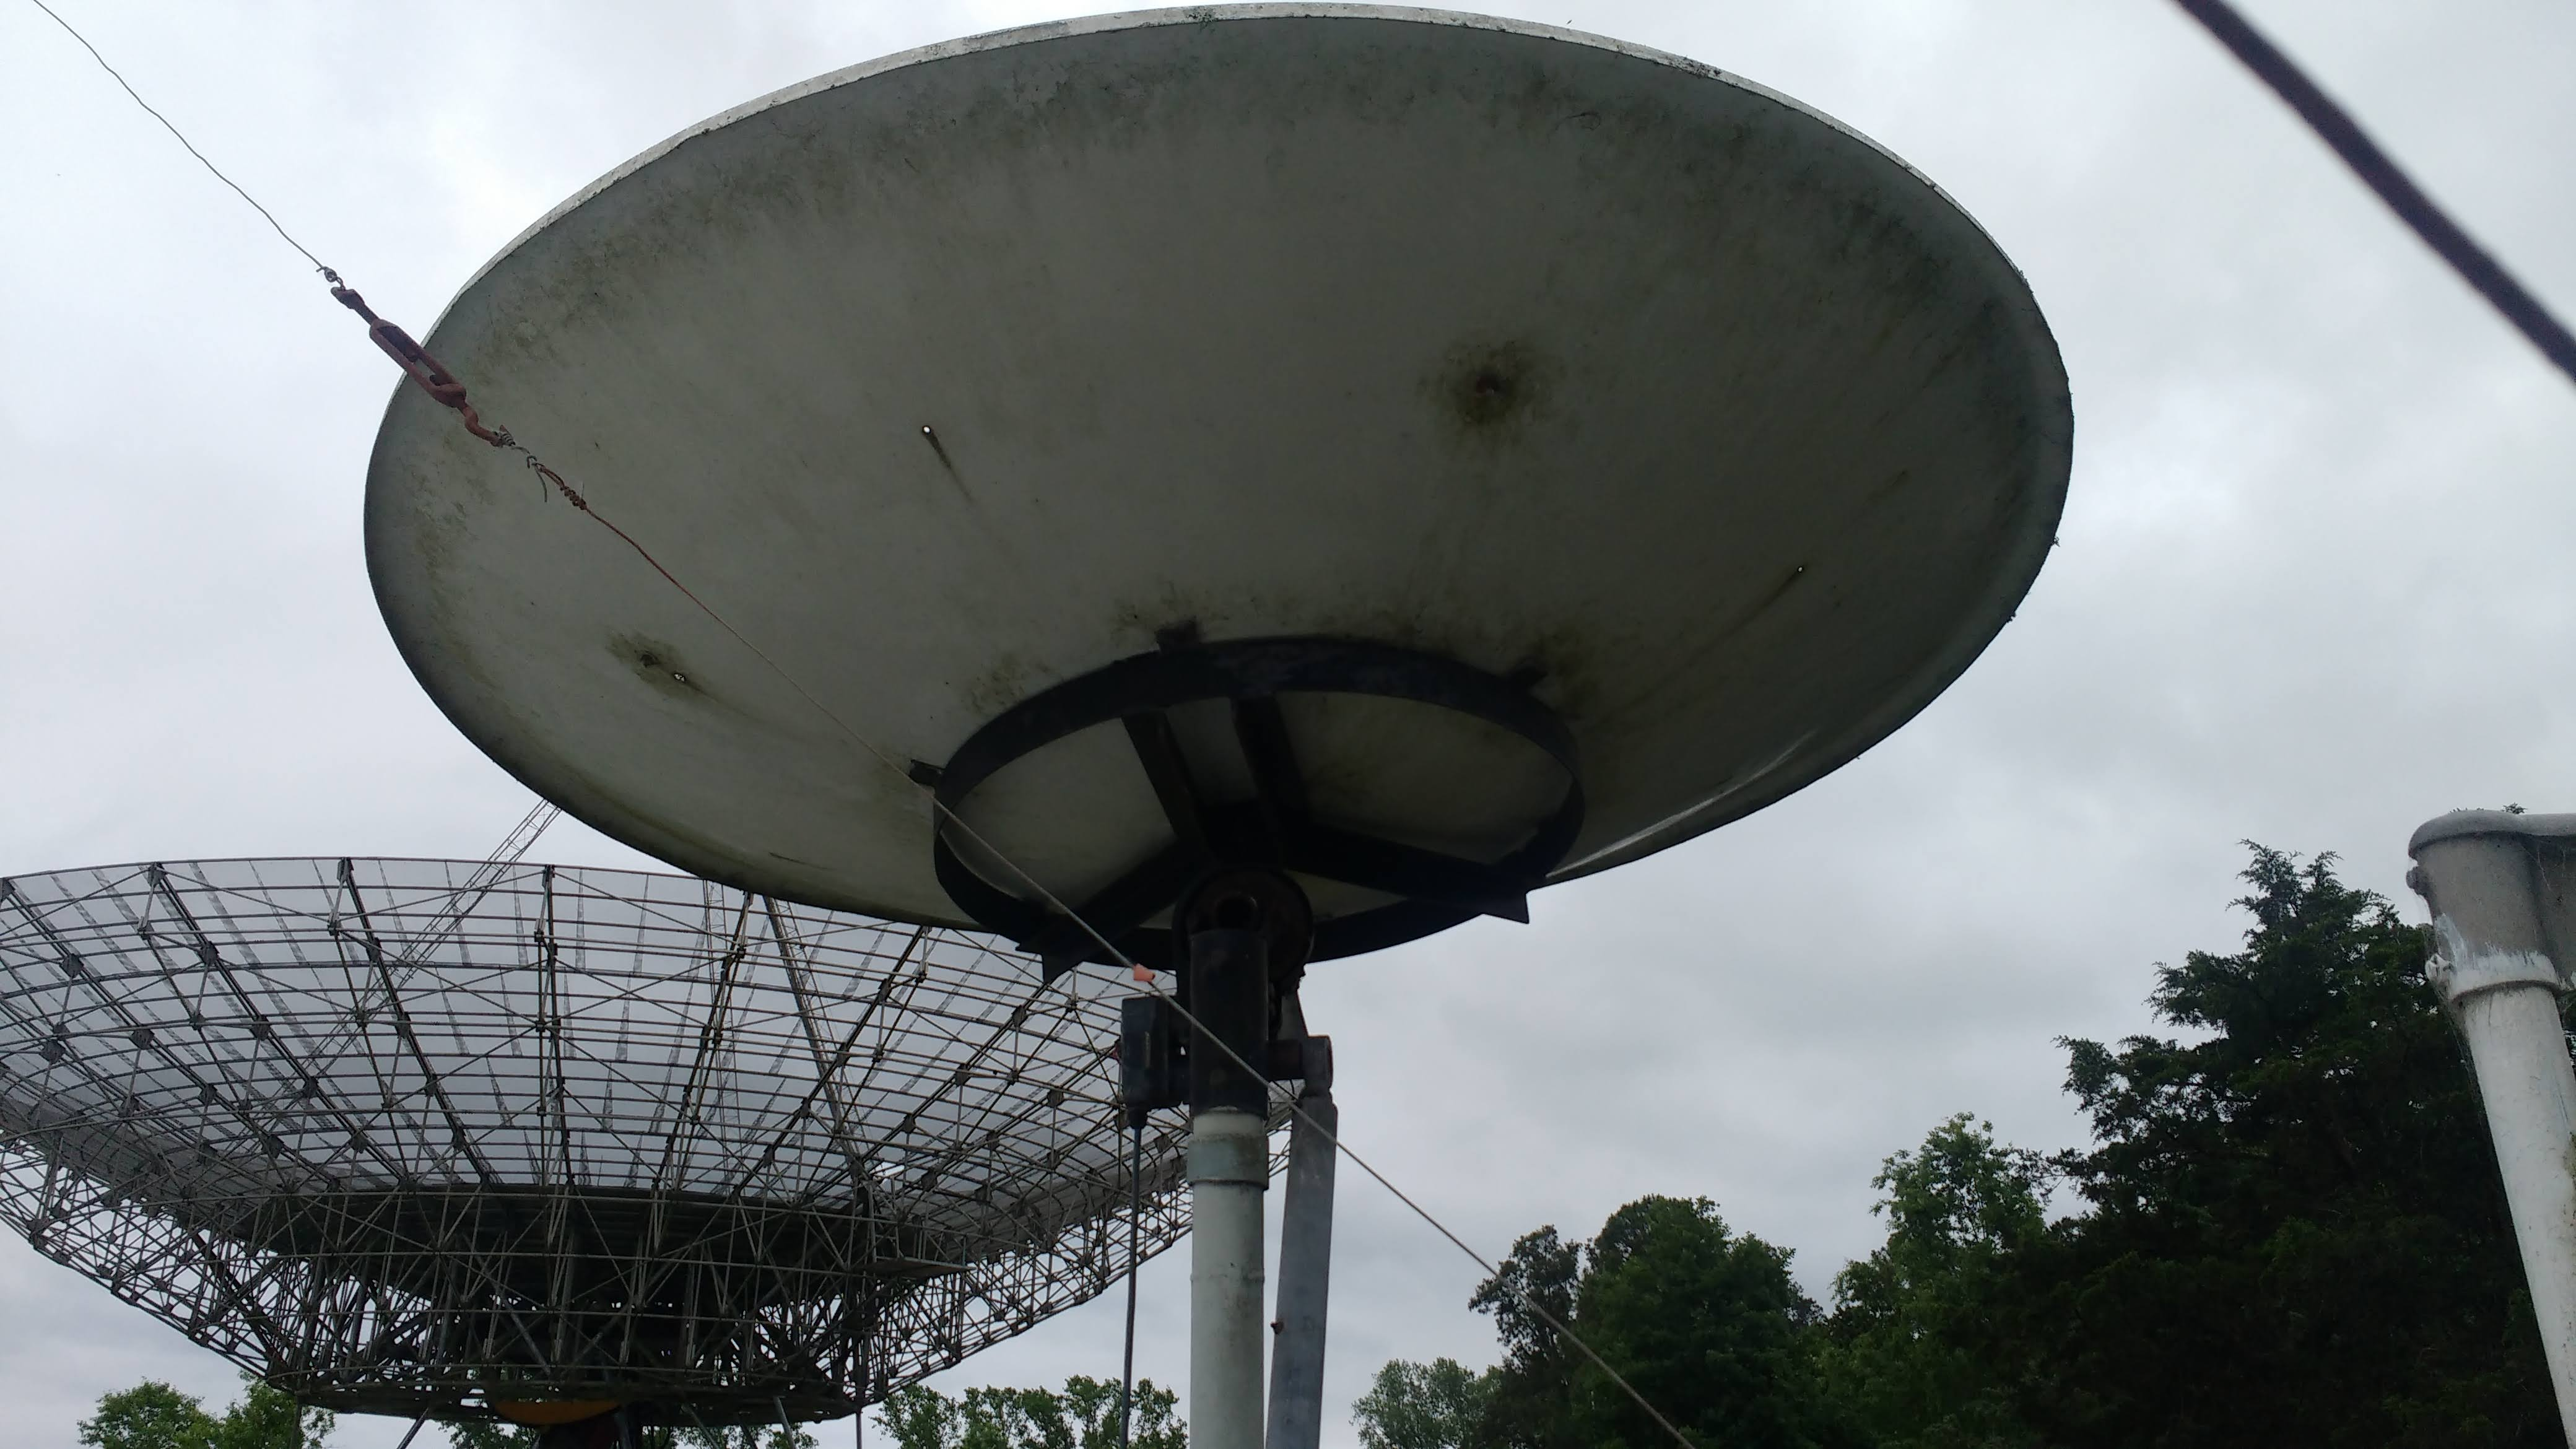
\includegraphics[width=0.5\textwidth]{parte_1/cap1/antena}
	\caption{antena ubicada en el iar, actualmente en desuso}
	\label{fig_antena}
\end{figure}

\section{Descripción de la Antena y posicionador }

La antena tiene el sistema mecánico que se observa en la figura \ref{fig_mec_ant}. 
% iamgen de la mecánica de la antena 
\begin{figure}[ht]
	%\centering 
	\begin{subfigure}{0.5\textwidth}
		\centering
		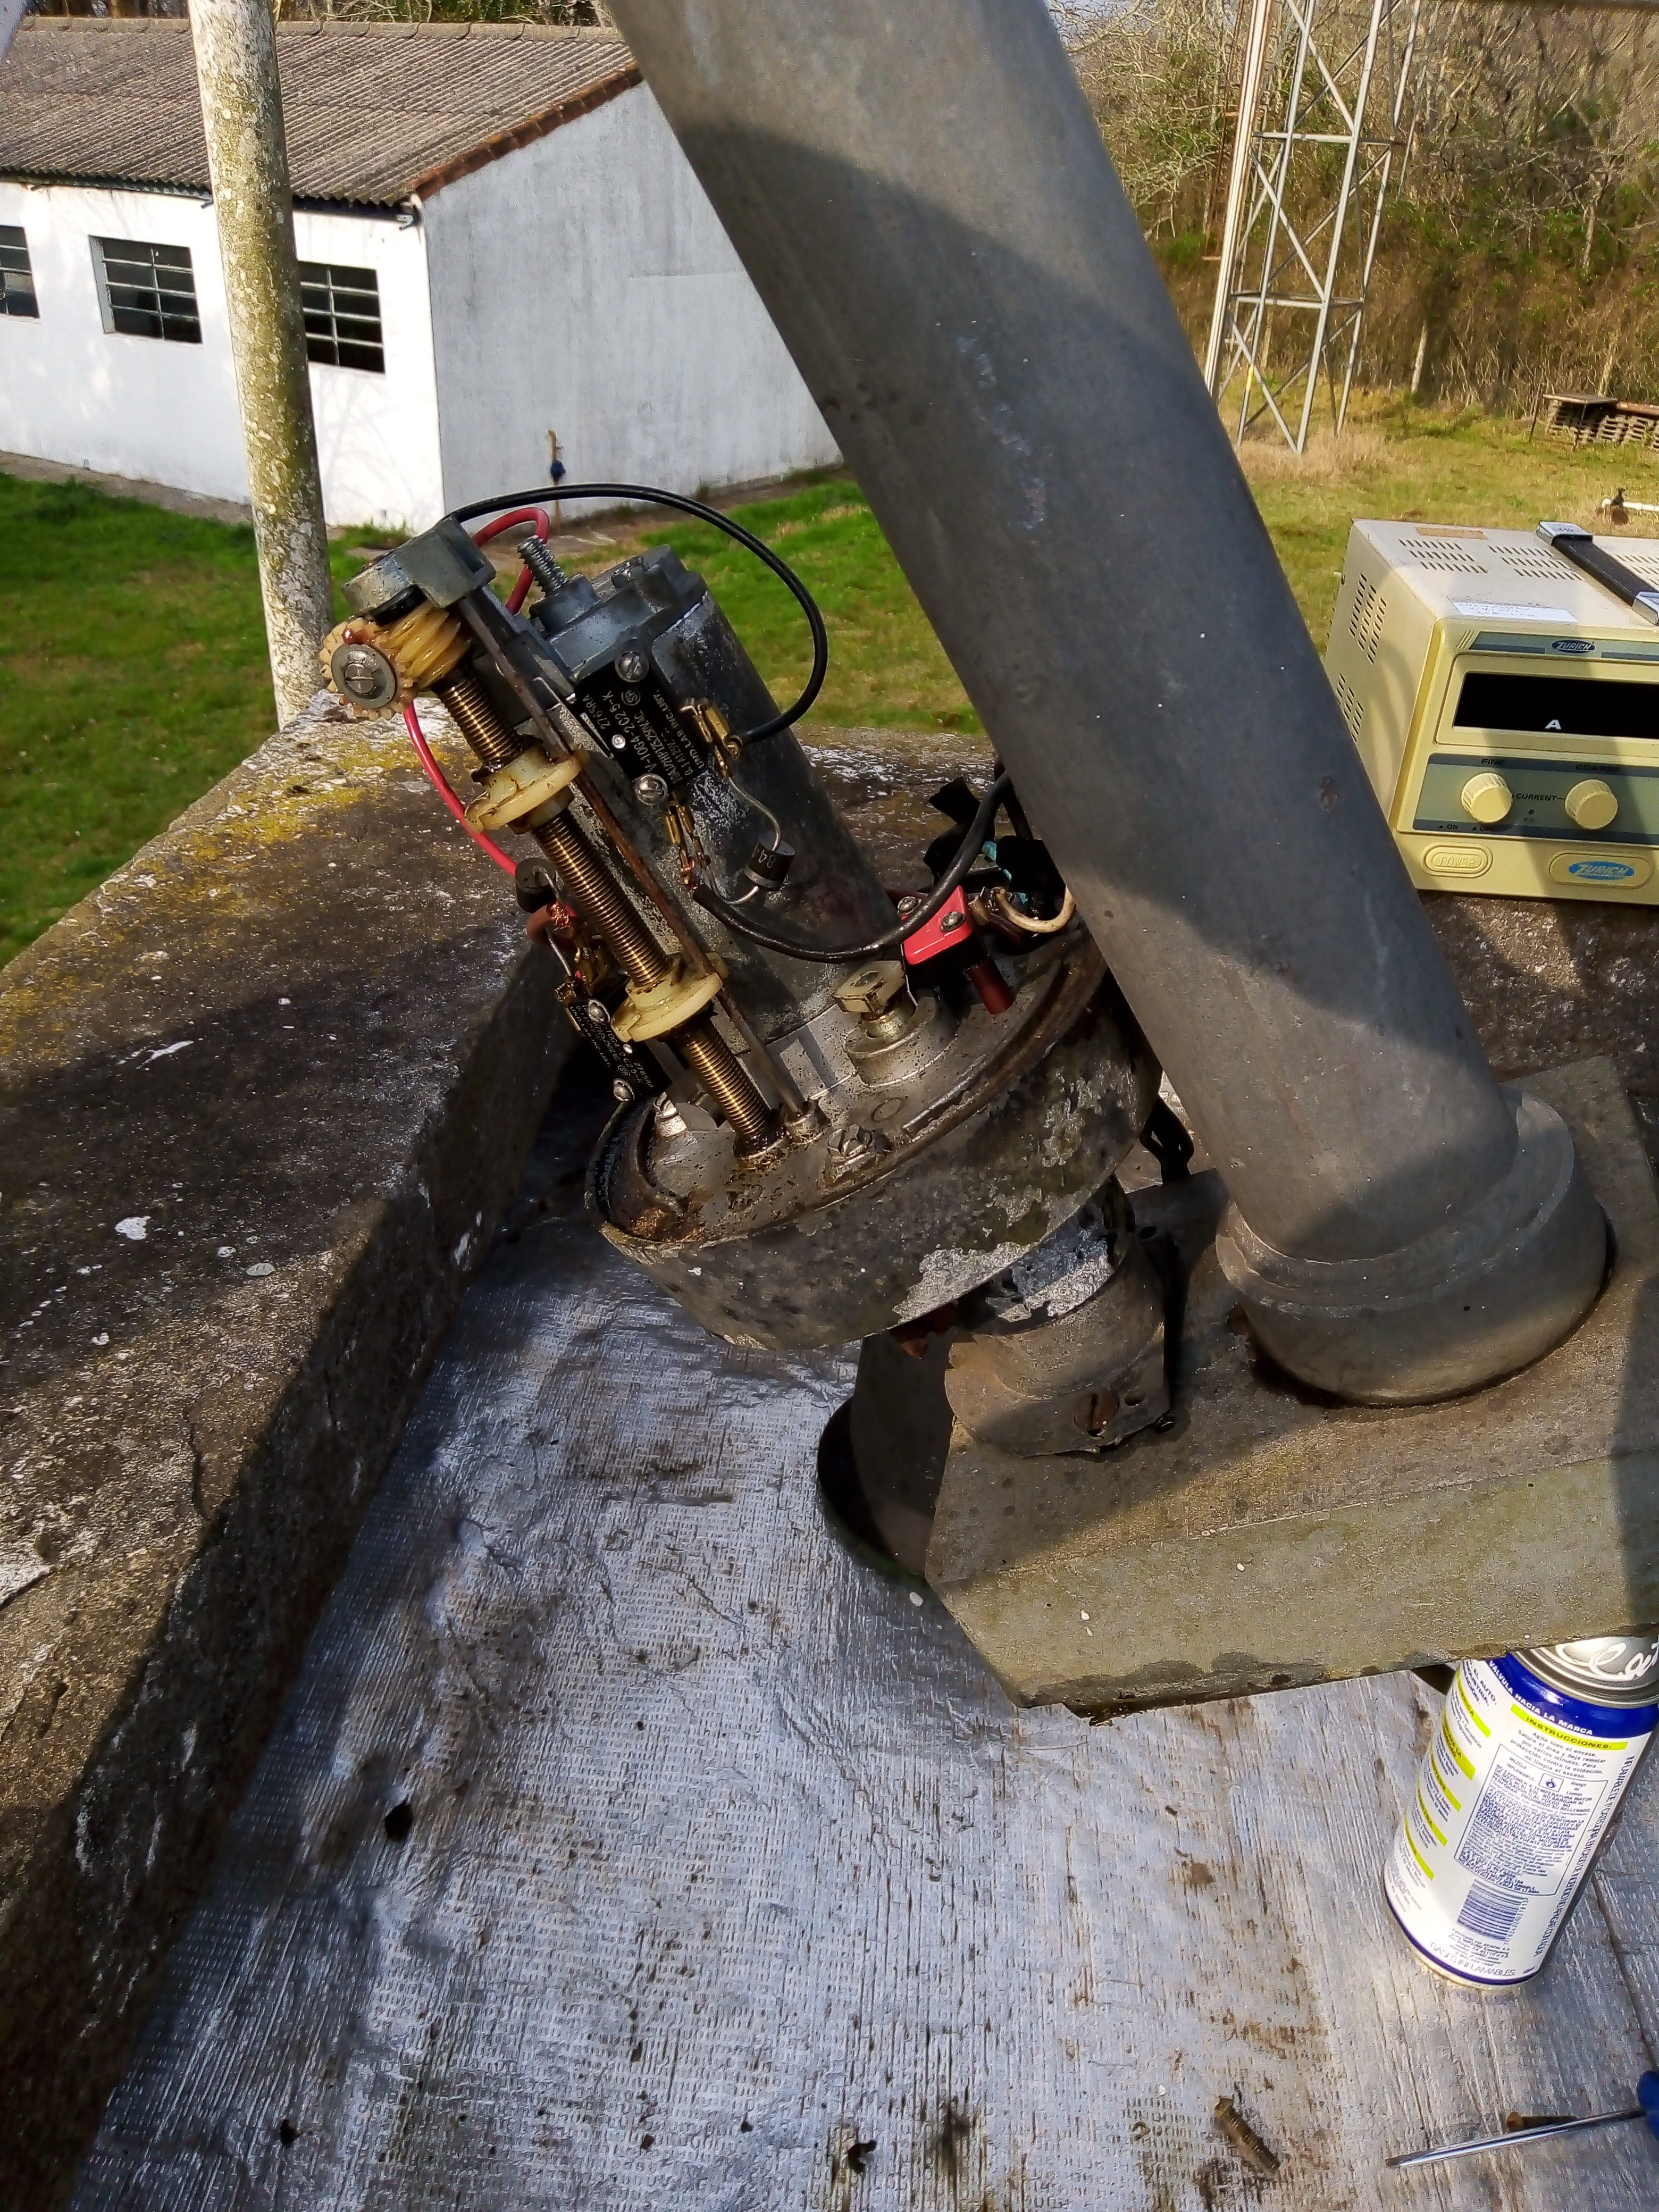
\includegraphics[width=0.5\textwidth]{parte_1/cap1/mot1}
		\caption{Motor de primer eje de la antena }
		\label{fig_mec_ant1}		
	\end{subfigure}
	\hfill 
	\begin{subfigure}{0.5\textwidth}
		\centering
		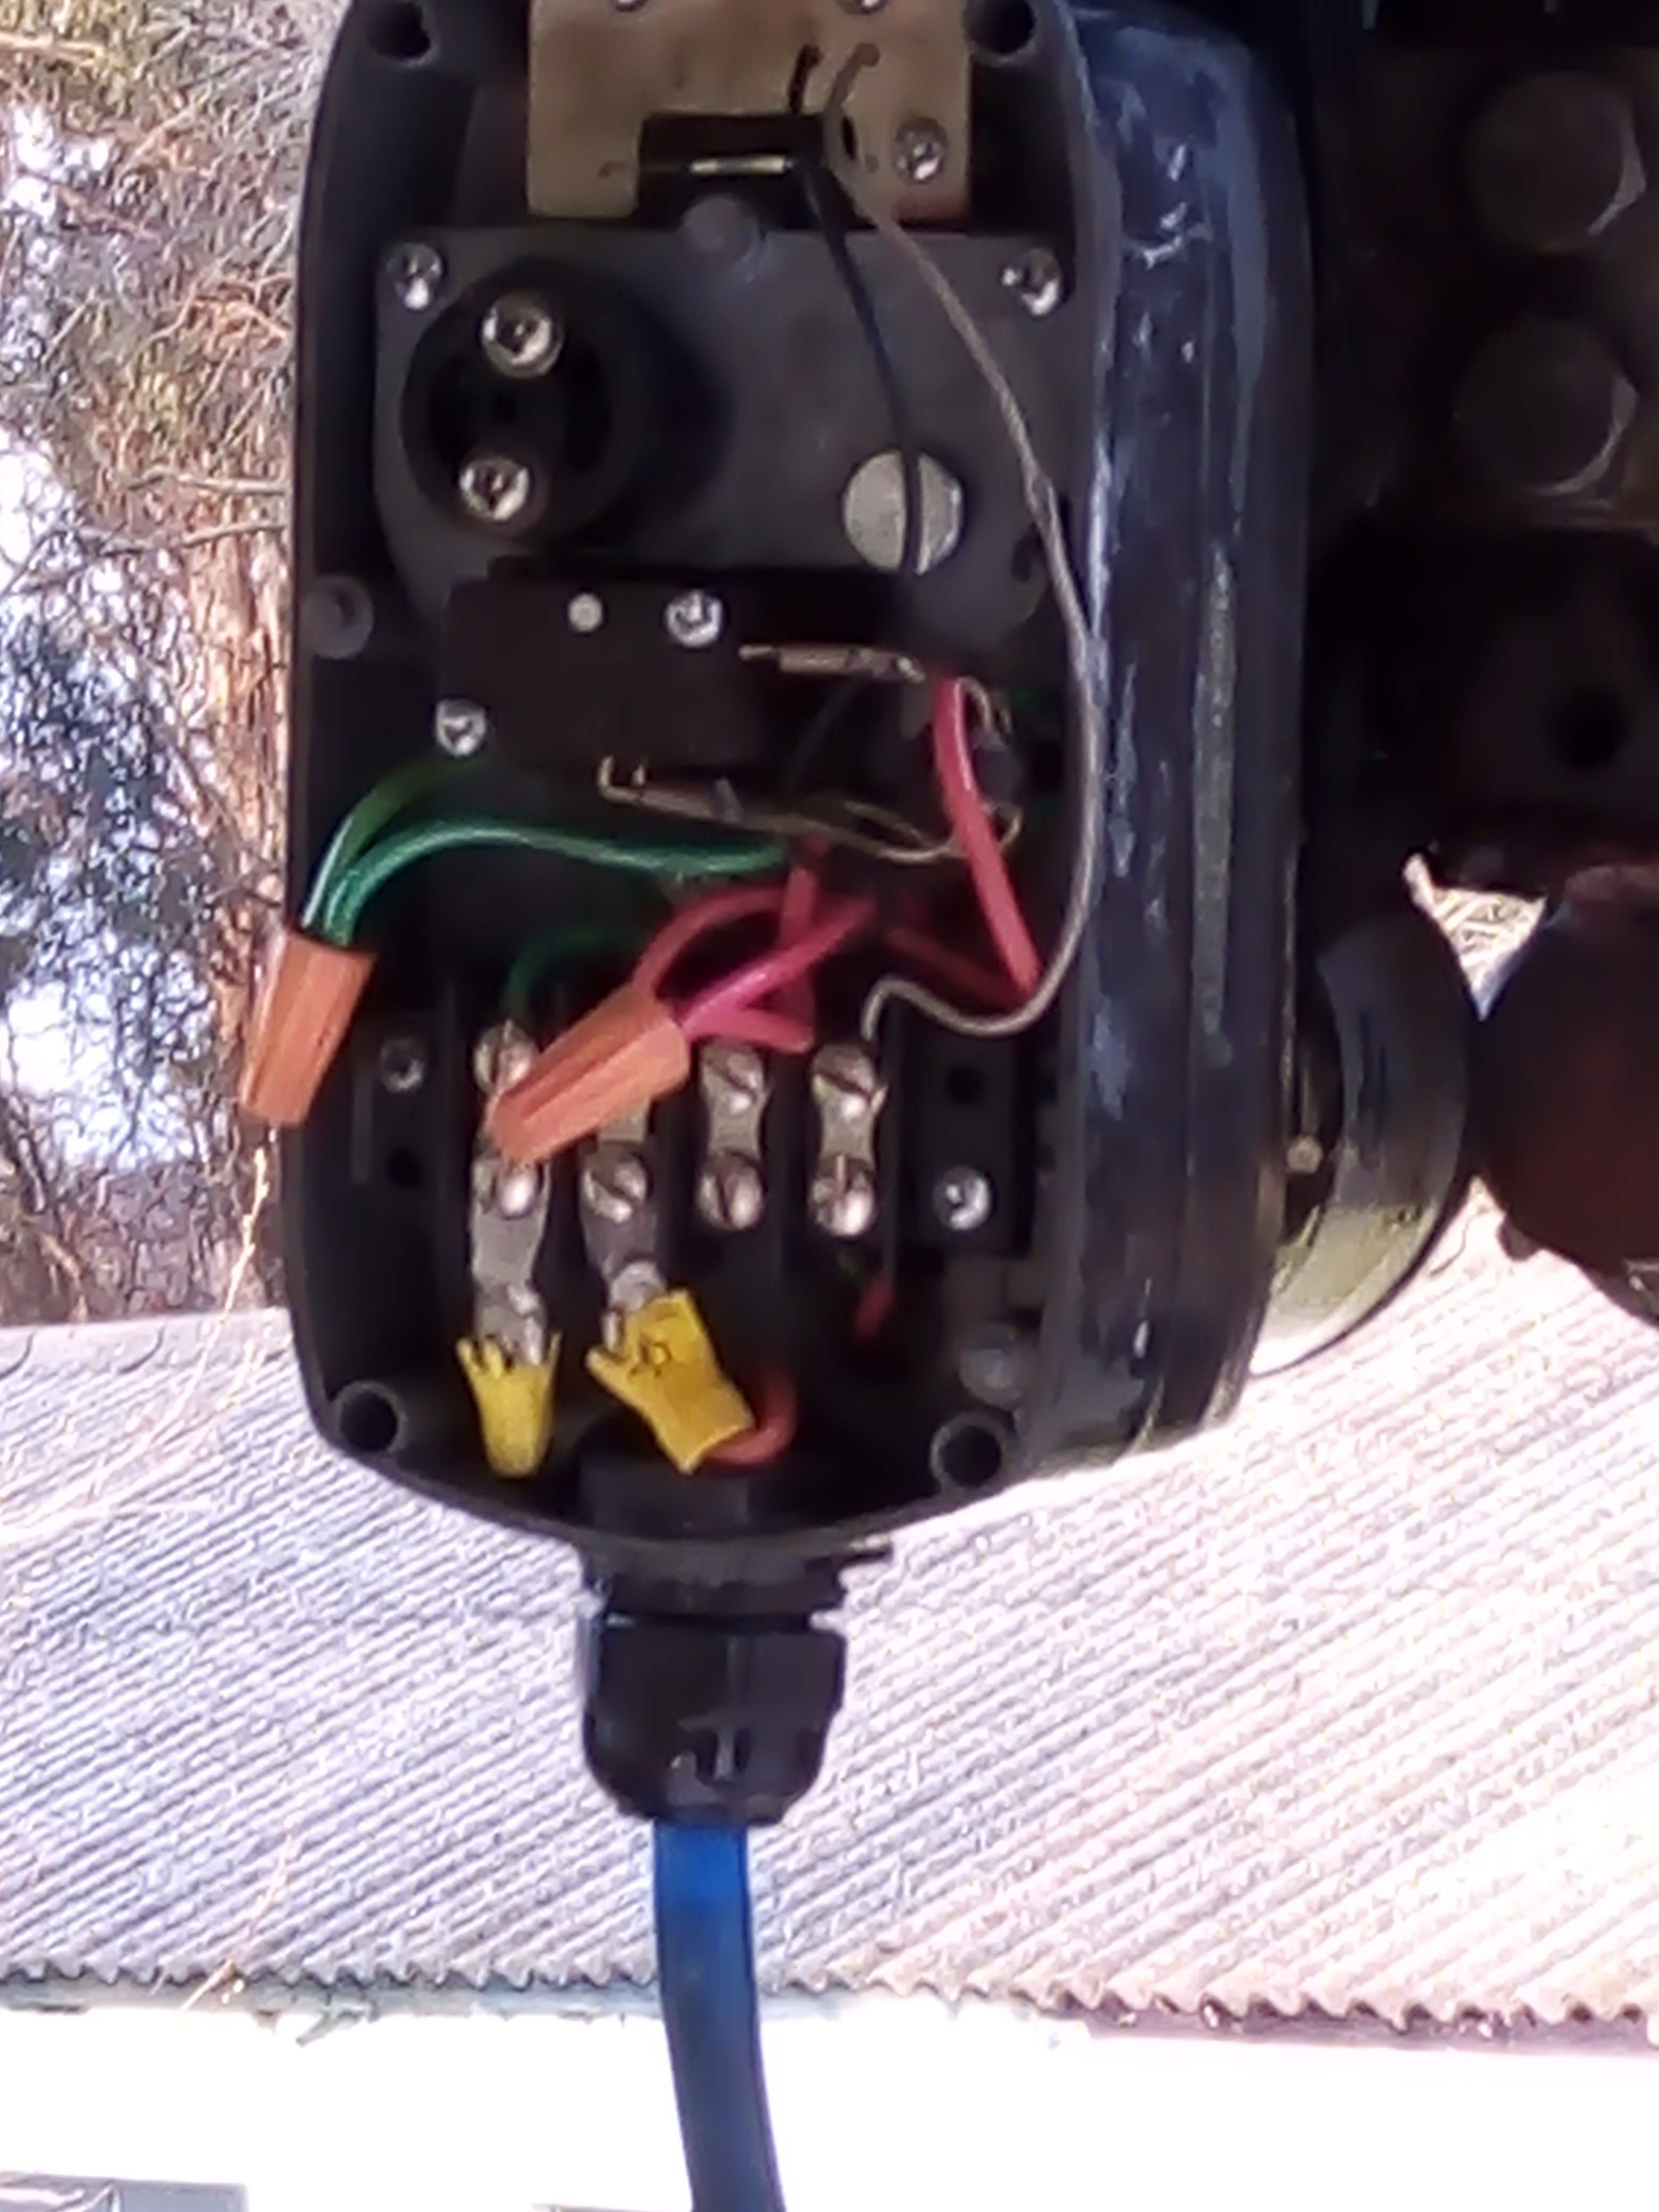
\includegraphics[width=0.5\textwidth]{parte_1/cap1/mot2}
		\caption{Motor de segundo eje de la antena }
		\label{fig_mec_ant2}
	\end{subfigure}
	
	\caption{antena ubicada en el iar, actualmente en desuso}
	\label{fig_mec_ant}
\end{figure}


En ella, se observa, que existen dos motores, uno para cada eje,además, tiene un sistema que permite medir la posición de la antena mediante dos potenciometros adosados al eje de cada motor. Estos ejes son independientes entre si,y su medida también. 



En el presente trabajo, se va a desarrollar un sistema que sea capaz de realizar el movimiento de la antena, aprovechando el sistema de motores existente sobre la misma. El sistema, que realiza el movimiento de la antena, se conoce como ''posicionador''. Este sistema, recibe una posición, en dos coordenadas, y tiene que mover la antena hacia esas coordenadas recibidas. Estas coordenadas recibidas, son las posiciones de los satélites, los cuales se van moviendo, por ende, mientras el satelite este por encima de la antena, o su ''horizonte visible'', debe realizar el seguimiento de la misma, actuando sobre los motores, y acomodando la antena, a donde este el satelite en cuestión.

En la actualidad, existen diversos software para realizar el seguimiento de satelites en tiempo real, estos consultan bases de datos existentes en internet, y realizan el cálculo en base a modelos matemáticos. En este documento, se hara uso de estos software, para poder actualizar la posición a cada instante y mover los motores hacia donde corresponda. Además, este dispositivo, debe ser controlador desde una PC que esté ubicada dentro de la institución. 

\section{Metodologia de trabajo}

El trabajo, se va a dividir en cuatro etapas, denominadas ''fase 1, fase 2,fase 3 y fase 4'' respectivamente. En la primera fase, se va a definir los requerimientos del sistema(capítulo actual), luego se va a proponer una solución a para cumplir estos requerimientos(cap. 2 ), y luego se van a seleccionar algunas piezas electrónicas para la construcción de la solución(cap 3.). 

En la segunda fase, se va a desarrollar el software que debe realizar el sistema de control, tanto para el usuario, como para la computadora que controla la antena. El orden del trabajo, es primero desarrollar el software sobre la computadora, y luego buscar interfaces disponibles, para conectarnos con ese equipo mediante el uso de internet. 



En la tercera fase, se va a realizar una investigación sobre los sistemas de coordenadas, como realizar las transformaciones de estas entre si, y la física de los satelites y modelos matemáticos.

En la cuarta fase, se va a desarrollar el sistema de posicionamiento de los motores, luego se desarrolla la interfaz para conectarse a la computadora que realiza el control del sistema. Luego, una vez desarrollado estas interfaces, se prueba el sistema realizando algún seguimiento, sea a satelites, o a estrellas.  



















\section{ Requerimientos del sistema} \label{req_sist}

De lo expuesto en las secciones anteriores, podemos obtener los requerimientos para este proyecto. Los requerimientos para este proyecto se dividen en dos tipos:  
\begin{enumerate}
	\item Requerimientos Funcionales.  
	\item Requerimientos de sistema. 
\end{enumerate} 
Donde en el primero, se definen aquellas cosas relacionadas al comporamiento del dispositivo a diseñar, mientras el segundo, se refiere a como llevar a cabo la solución en si. 

%\renewcommand{\multirowsetup}{\centering}

\renewcommand{\arraystretch}{1.5}

\begin{table}[H]
\begin{tabular}{|c|c| p{10cm} | }
% REQUISITOS FUNCIONALES 
	 \hline 	 
	 \multirow{11}{*}[-0.5cm]{\rotatebox[origin=c]{90}{\centering Requerimientos}} 
	 &\multirow{5}{*}[-0.25cm]{\centering Requisitos funcionales} & Medir posición de la antena. \\ \cline{3-3}
	 & & Recibir coordenadas desde una PC dentro del IAR. \\ \cline{3-3}
	 & & Tener control sobre la posición de la antena.\\  \cline{3-3}
	 & & Estacionar la antena en la posición del Zenith cuando no realize       		seguimientos sobre satelites. \\    \cline{3-3}
	 & & Seguimiento de satelites, naturales y artificiales, y estrellas. \\ \cline{3-3}
	 \cline{2-3}
% REQUISITOS DE SISTEMA 
	 &\multirow{6}{*}[-0.4cm]{\centering Requisitos De Sistema} & No puede utilizar ningún tipo de red inalámbrica. \\ 
	 \cline{3-3}	
	 & & Existencia de componentes en el mercado local. \\
	 \cline{3-3}
	 & & Escalable. \\ \cline{3-3}  
	 & & Independencia entre los componentes del sistema. \\ \cline{3-3}
	 & & Calibración automática de sentido de movimiento y posiciones angulares. \\ \cline{3-3}
	 & & Manejo desde una PC dentro de la institución. \\ \cline{3-3}  
	 & & Bajo Costo. \\
	 \hline 
\end{tabular}
\caption{Requerimientos del sistema }
\label{tab:requerimientos}
\end{table}








% imagen de la antena La tabla anterior, nos brinda los requerimientos, sobre los cuales se va a desarrollar el sistema de posicionamiento para la antena en cuestion. Los requerimientos, están de acuerdo, a la necesidad de la institución. 





 

 
%------------Final capitulo 1 ------------------------------%  



